% !TEX TS-program = pdflatex
% !TEX encoding = UTF-8 Unicode

% Article template :)

% General stuff
\documentclass[11pt]{article} % use larger type; default would be 10pt

\usepackage[utf8]{inputenc} % set input encoding (not needed with XeLaTeX)
\usepackage[french]{babel} % Language setting
\usepackage [T1] {fontenc}
\pdfmapfile{Overpass.map}

% Geometry
\usepackage{geometry}
\geometry{a4paper}
\geometry{margin=2cm}

% Usefull packages
\usepackage{eso-pic} % to add background images to the article
\usepackage{graphicx} % support the \includegraphics command and options
%\usepackage[colorlinks=false]{hyperref}
\usepackage{titlesec} % to change default styles of /sections, /title ...
\usepackage{xcolor}
\usepackage{tabto}
%\usepackage{amssymb}
\usepackage{amssymb}
\usepackage{multirow}
\usepackage{tikz}
\usetikzlibrary{arrows,automata,positioning}
\usepackage{amsmath}
\usepackage{lettrine}
\usepackage{oldgerm}
\usepackage{yfonts}
\usepackage{multicol}
\usepackage{blindtext}
\usepackage{svg}
\usepackage{tabularx}
\usepackage{hyperref}
\hypersetup{
    colorlinks=true,
    linkcolor=blue,
    filecolor=magenta,
    urlcolor=cyan,
    pdftitle={Overleaf Example},
    pdfpagemode=FullScreen,
    }

\newcommand{\enluminure}[2]{\lettrine[lines=3]{\small \initfamily #1}{#2}}


% Style !
\definecolor{10Black}{cmyk}{0, 0, 0, 0.10} % 10% of black
\definecolor{20Black}{cmyk}{0, 0, 0, 0.20} % 20% of black
\definecolor{80Black}{cmyk}{0, 0, 0, 0.80} % 80% of black
\definecolor{95Black}{cmyk}{0, 0, 0, 0.95} % 60% of black
%\color{10Black}
%\pagecolor{black}

% New commands
\newcommand{\myjump}[1][1]{\mbox{}\\[#1cm]}


\begin{document}
\pagestyle{empty}

\begin{center}
    \textbf{Petit JDR universel}

    Règles de base
\end{center}

\enluminure{P}{eut} importe la quantité de règles qu'un jdr offre, on attendras toujours du MJ qu'il juge les situations non régulés, qu'il improvise et applique la règle du cool. Le petit JDR universel propose peu de règles, il se repose sur les accords qui existes entre joueurs et MJ.


\myjump[0]
\textbf{\huge Joueurs}


\myjump[0]
\textbf{Feuille de personnages}


\noindent
\begin{tabularx}{\textwidth}{cXcX}
\hline
    \scalebox{0.92}{
\includegraphics{images/heart.png}} & PV max + 1 &
    \scalebox{0.05}{
\includegraphics{images/chestplate.png}} & Defense max + 1\\

    \scalebox{0.03}{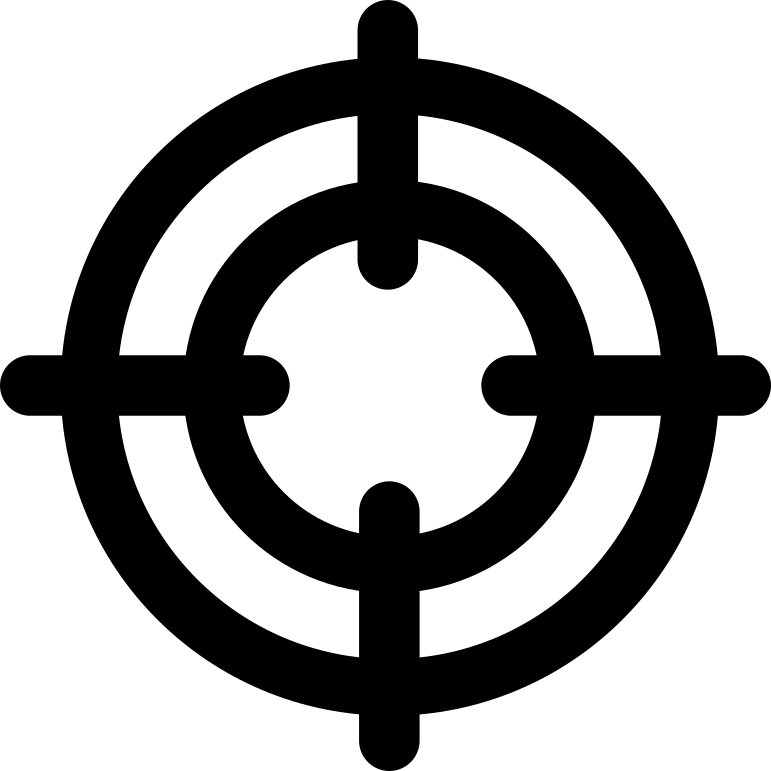
\includegraphics{images/cible.png}} & Objectif de Combat (OC) - 1 &
    \scalebox{0.025}{
\includegraphics{images/sword.png}} & Augmente le bonus de dégâts\\


    \scalebox{0.03}{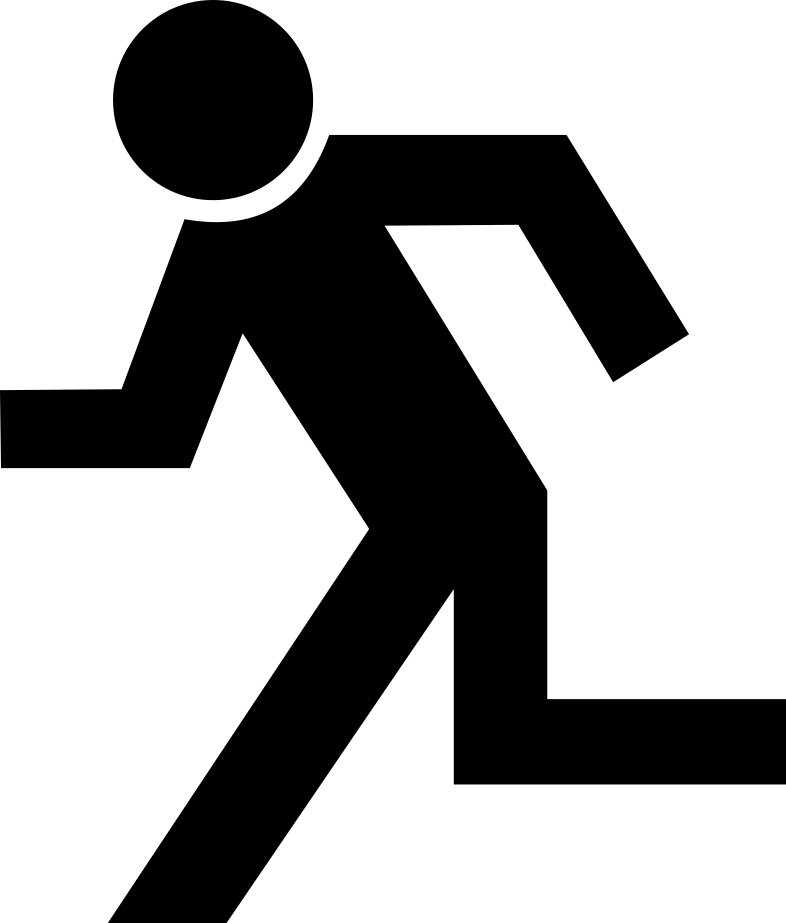
\includegraphics{images/esquive.png}} & Esquive + 1, l'esquive augemente de 1 l'OC d'un ennemy vous attaquant&
    \scalebox{0.015}{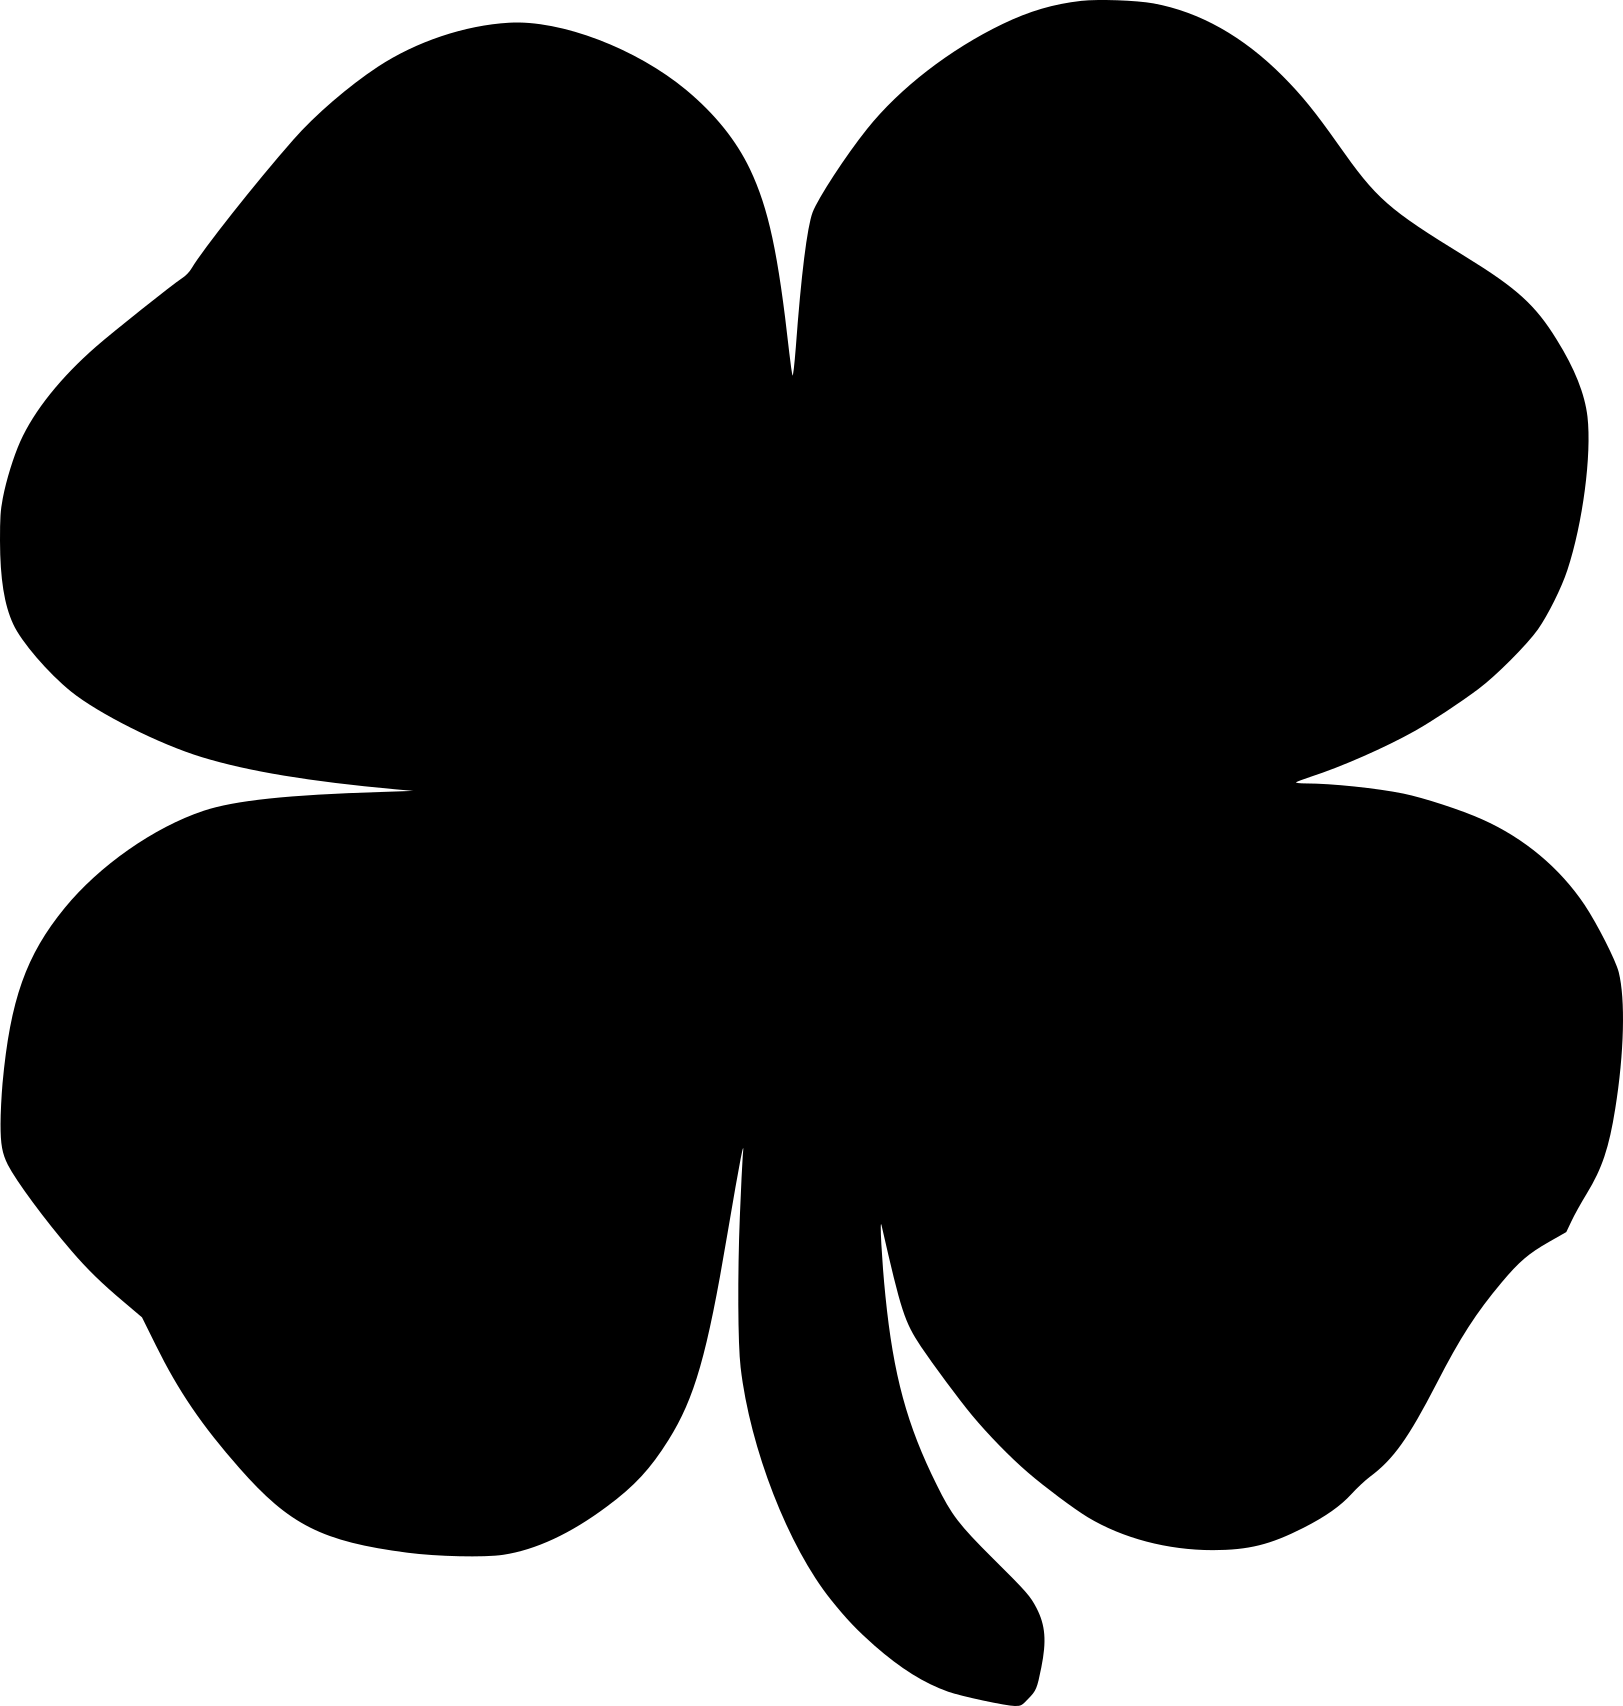
\includegraphics{images/chance.png}} & Chance + 1, un point de chance permet de relancer un dés. Le MJ décide quand est-ce que les points de chance se reset\\


    \vspace{0.3cm}\scalebox{0.065}{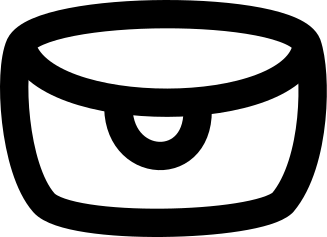
\includegraphics{images/pouch.png}} & \multicolumn{3}{@{}l}{Augmente de 1 le nombre d'armes pouvant être portées et utilisés sans malus en combat}\\

\hline
    \textbf{PV} &Lorsque le personnage atteint 3 PV, il recoit une blessure grave décrite par le MJ et le besoin de s'alliter un certain nombre de jours (?) &
    \textbf{Stress} & Par défaut à 0/6, augmenté par le MJ. Stress au delas du niveau 6 est à la discrétion du MJ\\
\hline
\end{tabularx}

\myjump[0.35]
\textbf{Compétences}\newline
À part dans l'arbre de progression, il n'existe pas de compétences pré-définies, c'est au joueur d'imaginer les compétences que son personnage possède. Pour réaliser des actions hors combat, le joueur doit justifier au MJ pourquoi son personnage est capable de réaliser la tache envisagée. Cette justification peut utiliser comme argument l'une des compétences du personnage.\newline
\begin{tabularx}{\linewidth}{|X}
\emph{\og J'aimerais que mon personnage cherche du cerfeuille dans la forêt. Il devrait en être capable d'en trouver car il a été élève d'un druide et possède la compétence herboristerie 2. \fg}\\
\end{tabularx}



\myjump[0.35]
\textbf{Création de personnage}\newline
Distribuer 10 points d'expérience dans l'arbre de progrésion. 6 points de connaissances sont disponibles et peuvent être distribués plus tard dans la partie. 4 de défense max. Équipement de départ à discuter avec le MJ.

\myjump[0]
\textbf{Combat}\newline
En combat, votre personnage peut réaliser 2 actions diférentes.
Lorsque votre personnage veut attaquer, il n'y a qu'un seul jet de dés à faire pour connaître les dégats qu'il infligera. Vous lancez 2d6 explosifs que vous comparez à votre Objectif de Combat (OC). Si le résultat est supérieur ou égal à  votre OC, vous additionez au jet de dés les dégats bonus de votre arbre et les dégats de votre arme.

$$
\mbox{Dégâts infligés} =
\left\{
    \begin{array}{ll}
        (2d6 \ge \mbox{OC}) + \mbox{bonnus degâts arbre} + \mbox{dégats arme}\\
(2d6 < \mbox{OC})
    \end{array}
\right.
$$

\noindent
\begin{tabularx}{\linewidth}{|X}
\emph{Biglour utilise sa dague qui fait 4 de dégats. Il a débloqué 2 cibles dans son arbre alors son Objectif de Combat (OC) vaut 12-2=10. Il a aussi atteint 2 épées et a donc 2 dégats bonus.
Il lance 2 dés 6 et obtient un 3 et un 6, le dés qui a atteint 6 explose et Biglour lance un dés supplémentaire qui fait 4. $3 + 6 + 4 = 13 \ge 10$ c'est suppérieur à son OC, il inflige donc $13 + 2 + 4 = 19$ de dégats. Au tours suivant il obtient $3 + 4 = 7 < 10$ et inflige 7 dégats}\\
\end{tabularx}










\newpage
\textbf{\huge Maître du Jeu}

\enluminure{L}{'improvisation} ne peut pas être utilisé pour solidifier du gameplay. Si la magie fait partie de votre univers mais qu'il n'y a pas de règles qui explique son fonctionement; alors cette magie est un outil scénaristique pour le MJ plutôt qu'un élément de gameplay pour les joueurs.

\myjump[0]
\textbf{Modules}\newline
\noindent Pour ajouter des éléments de gameplay au set de règles de ce jeu de rôle, vous pouvez ajourter des modules que vous retrouverez sur la page suivante : \href{https://github.com/kalharko/petit-jdr-universel}{github.com/kalharko/petit-jdr-universel}.



\myjump[0]
\textbf{Compétences}\newline
Le cadre de \emph{compétence} de la feuille de personnage recueille tous les domaines où le personnage possède une maitrise ou un savoir. Pour réaliser des actions hors combat, les joueurs vont justifier pourquoi leur personnage est capable de réaliser la tache envisagée. Vous devez juger leur argumentaire en prenant en compte les compétences du personnage, sa condition et l'histoire. Les domaines techniques sont très faciles à juger, quelqu'un qui ne s'est jamais entrainé au crochetage, ne peut pas crocheter. Pour les situations plus nuancés le MJ doit prendre en compte l'histoire et choisir le jugement qui va ajouter le plus de drame et de rebondissement à l'histoire.\newline\newline
\begin{tabularx}{\linewidth}{|X}
\emph{Biglour veut s'introduire dans les archives de la guilde marchande. Grâce à sa compétence crochetage 2, Biglour a prévu de s'introduire par une porte de service. Mais il a alerté la garde sur son chemin et doit maintenant se dépécher de crocheter. Le MJ estime que les archives sont protégés par des serrures de bonne facture et Biglour aurais mis du temps à crocheter. Le MJ doit juger quelle issue offre le plus de drame, d'interêt pour les joueurs et de ramifications futur à l'histoire : échapper de peu à la garde et continuer sa mission, ou devoir confronter la garde immédiatement. }\\
\end{tabularx}
\myjump[0.35]
Pour entrainer des compétences, les joueurs doivent trouver un personnage dans le jeu pour les aider à apprendre et investir du temps dans leur entrainement.

\myjump[0]
\textbf{Combat}\newline
En combat les dégats des forces opposant les joueurs sont calculés ainsi :

\noindent
\begin{tabular}{c|c}
    1d6 $\ge$ 2 + esquive de la cible & dégats haut \\
    1d6 $<$ 2 + esquive de la cible & dégats bas \\
\end{tabular}



\myjump[0.4]\noindent
Les armes de bases font entre 2 et 4 dégâts, à chaque fois qu'un joueur trouve une nouvelle arme, elle devrait faire 2 dégâts de plus.

\begin{tabularx}{\textwidth}{cX|cX}
    \sc{\textbf{Armes}} & & \sc{\textbf{Créatures}} &\\
    Épée & 5 dégats & Goblin & 8-14 dégats; 10 pv\\
    Marteau & 6 dégats & Troll & testest\\
    Arc & 4 dégats & Griphon & testest\\
    Flèche & 3 dégats & Slime & testes\\


\end{tabularx}





\newpage
\begin{center}
\textbf{Distribution 2d6}
\myjump
\begin{tabular}{c|c|c|c|c|c|c|}
     & 1& 2& 3& 4& 5& 6\\\cline{2-7}
    1& 2& 3& 4& 5& 6& 7\\\cline{2-7}
    2& 3& 4& 5& 6& 7& 8\\\cline{2-7}
    3& 4& 5& 6& 7& 8& 9\\\cline{2-7}
    4& 5& 6& 7& 8& 9&10\\\cline{2-7}
    5& 6& 7& 8& 9&10&11\\\cline{2-7}
    6& 7& 8& 9&10&11&12\\\cline{2-7}
\end{tabular}

\myjump
\begin{tabular}{c|ccccccccccc}
      17\%&  &  &  &  &  & -&  &  &  &  &  \\
      14\%&  &  &  &  & -& -& -&  &  &  &  \\
      11\%&  &  &  & -& -& -& -& -&  &  &  \\
       8\%&  &  & -& -& -& -& -& -& -&  &  \\
     5.5\%&  & -& -& -& -& -& -& -& -& -&  \\
        \%& -& -& -& -& -& -& -& -& -& -& -\\
        \%& 2& 3& 4& 5& 6& 7& 8& 9&10&11&12\\

\end{tabular}
\end{center}


TODO
\begin{itemize}
    \item ajouter au scenario le fait qu'ils ont plus d'argent à cause du prix d'entré du tournois
    \item dessiner la carte du sous sol
    \item designer la reine insectes (glyphe sur l'abdomen)
    \item ouvriers, guerrier, bouclier(volant oneshot), kamikaze qui paralise
    \item finir le module d'enchantement
    \item ecrire description épée electrique (forte mais fait beaucoup de bruit)
    \item comment créer un coup spécial

    \item coup spécial : pas 2 fois sur le même groupe d'ennemi
\end{itemize}


\begin{itemize}
    \item combien dé nnemi ca touche
    \item est-ce-que stress +1
    \item effet sur cible
    \item
    \item effet negatif sur utilisateur
    \item
    \item attaque
    \item attaque dans le dos = +1d6
    \item 2 cibles = degats complet et degats /2 1fois
    \item 3 ou plus cibles = degats/2 1fois
    \item
    \item defense = +3 def pendant un tour 1fois
    \item fuite = donne du déplacement 1fois
    \item
    \item stun 1 fois
    \item charge = degats/2 1 fois
    \item pousser 1 fois
    \item augmenter oc cible
    \item cracheur de feu = attaque normale
    \item
    \item provocation n'est pas un coup spécial

\end{itemize}

\end{document}
